\documentclass[1p]{elsarticle_modified}
%\bibliographystyle{elsarticle-num}

%\usepackage[colorlinks]{hyperref}
%\usepackage{abbrmath_seonhwa} %\Abb, \Ascr, \Acal ,\Abf, \Afrak
\usepackage{amsfonts}
\usepackage{amssymb}
\usepackage{amsmath}
\usepackage{amsthm}
\usepackage{scalefnt}
\usepackage{amsbsy}
\usepackage{kotex}
\usepackage{caption}
\usepackage{subfig}
\usepackage{color}
\usepackage{graphicx}
\usepackage{xcolor} %% white, black, red, green, blue, cyan, magenta, yellow
\usepackage{float}
\usepackage{setspace}
\usepackage{hyperref}

\usepackage{tikz}
\usetikzlibrary{arrows}

\usepackage{multirow}
\usepackage{array} % fixed length table
\usepackage{hhline}

%%%%%%%%%%%%%%%%%%%%%
\makeatletter
\renewcommand*\env@matrix[1][\arraystretch]{%
	\edef\arraystretch{#1}%
	\hskip -\arraycolsep
	\let\@ifnextchar\new@ifnextchar
	\array{*\c@MaxMatrixCols c}}
\makeatother %https://tex.stackexchange.com/questions/14071/how-can-i-increase-the-line-spacing-in-a-matrix
%%%%%%%%%%%%%%%

\usepackage[normalem]{ulem}

\newcommand{\msout}[1]{\ifmmode\text{\sout{\ensuremath{#1}}}\else\sout{#1}\fi}
%SOURCE: \msout is \stkout macro in https://tex.stackexchange.com/questions/20609/strikeout-in-math-mode

\newcommand{\cancel}[1]{
	\ifmmode
	{\color{red}\msout{#1}}
	\else
	{\color{red}\sout{#1}}
	\fi
}

\newcommand{\add}[1]{
	{\color{blue}\uwave{#1}}
}

\newcommand{\replace}[2]{
	\ifmmode
	{\color{red}\msout{#1}}{\color{blue}\uwave{#2}}
	\else
	{\color{red}\sout{#1}}{\color{blue}\uwave{#2}}
	\fi
}

\newcommand{\Sol}{\mathcal{S}} %segment
\newcommand{\D}{D} %diagram
\newcommand{\A}{\mathcal{A}} %arc


%%%%%%%%%%%%%%%%%%%%%%%%%%%%%5 test

\def\sl{\operatorname{\textup{SL}}(2,\Cbb)}
\def\psl{\operatorname{\textup{PSL}}(2,\Cbb)}
\def\quan{\mkern 1mu \triangleright \mkern 1mu}

\theoremstyle{definition}
\newtheorem{thm}{Theorem}[section]
\newtheorem{prop}[thm]{Proposition}
\newtheorem{lem}[thm]{Lemma}
\newtheorem{ques}[thm]{Question}
\newtheorem{cor}[thm]{Corollary}
\newtheorem{defn}[thm]{Definition}
\newtheorem{exam}[thm]{Example}
\newtheorem{rmk}[thm]{Remark}
\newtheorem{alg}[thm]{Algorithm}

\newcommand{\I}{\sqrt{-1}}
\begin{document}

%\begin{frontmatter}
%
%\title{Boundary parabolic representations of knots up to 8 crossings}
%
%%% Group authors per affiliation:
%\author{Yunhi Cho} 
%\address{Department of Mathematics, University of Seoul, Seoul, Korea}
%\ead{yhcho@uos.ac.kr}
%
%
%\author{Seonhwa Kim} %\fnref{s_kim}}
%\address{Center for Geometry and Physics, Institute for Basic Science, Pohang, 37673, Korea}
%\ead{ryeona17@ibs.re.kr}
%
%\author{Hyuk Kim}
%\address{Department of Mathematical Sciences, Seoul National University, Seoul 08826, Korea}
%\ead{hyukkim@snu.ac.kr}
%
%\author{Seokbeom Yoon}
%\address{Department of Mathematical Sciences, Seoul National University, Seoul, 08826,  Korea}
%\ead{sbyoon15@snu.ac.kr}
%
%\begin{abstract}
%We find all boundary parabolic representation of knots up to 8 crossings.
%
%\end{abstract}
%\begin{keyword}
%    \MSC[2010] 57M25 
%\end{keyword}
%
%\end{frontmatter}

%\linenumbers
%\tableofcontents
%
\newcommand\colored[1]{\textcolor{white}{\rule[-0.35ex]{0.8em}{1.4ex}}\kern-0.8em\color{red} #1}%
%\newcommand\colored[1]{\textcolor{white}{ #1}\kern-2.17ex	\textcolor{white}{ #1}\kern-1.81ex	\textcolor{white}{ #1}\kern-2.15ex\color{red}#1	}

{\Large $\underline{12a_{0870}~(K12a_{0870})}$}

\setlength{\tabcolsep}{10pt}
\renewcommand{\arraystretch}{1.6}
\vspace{1cm}\begin{tabular}{m{100pt}>{\centering\arraybackslash}m{274pt}}
\multirow{5}{120pt}{
	\centering
	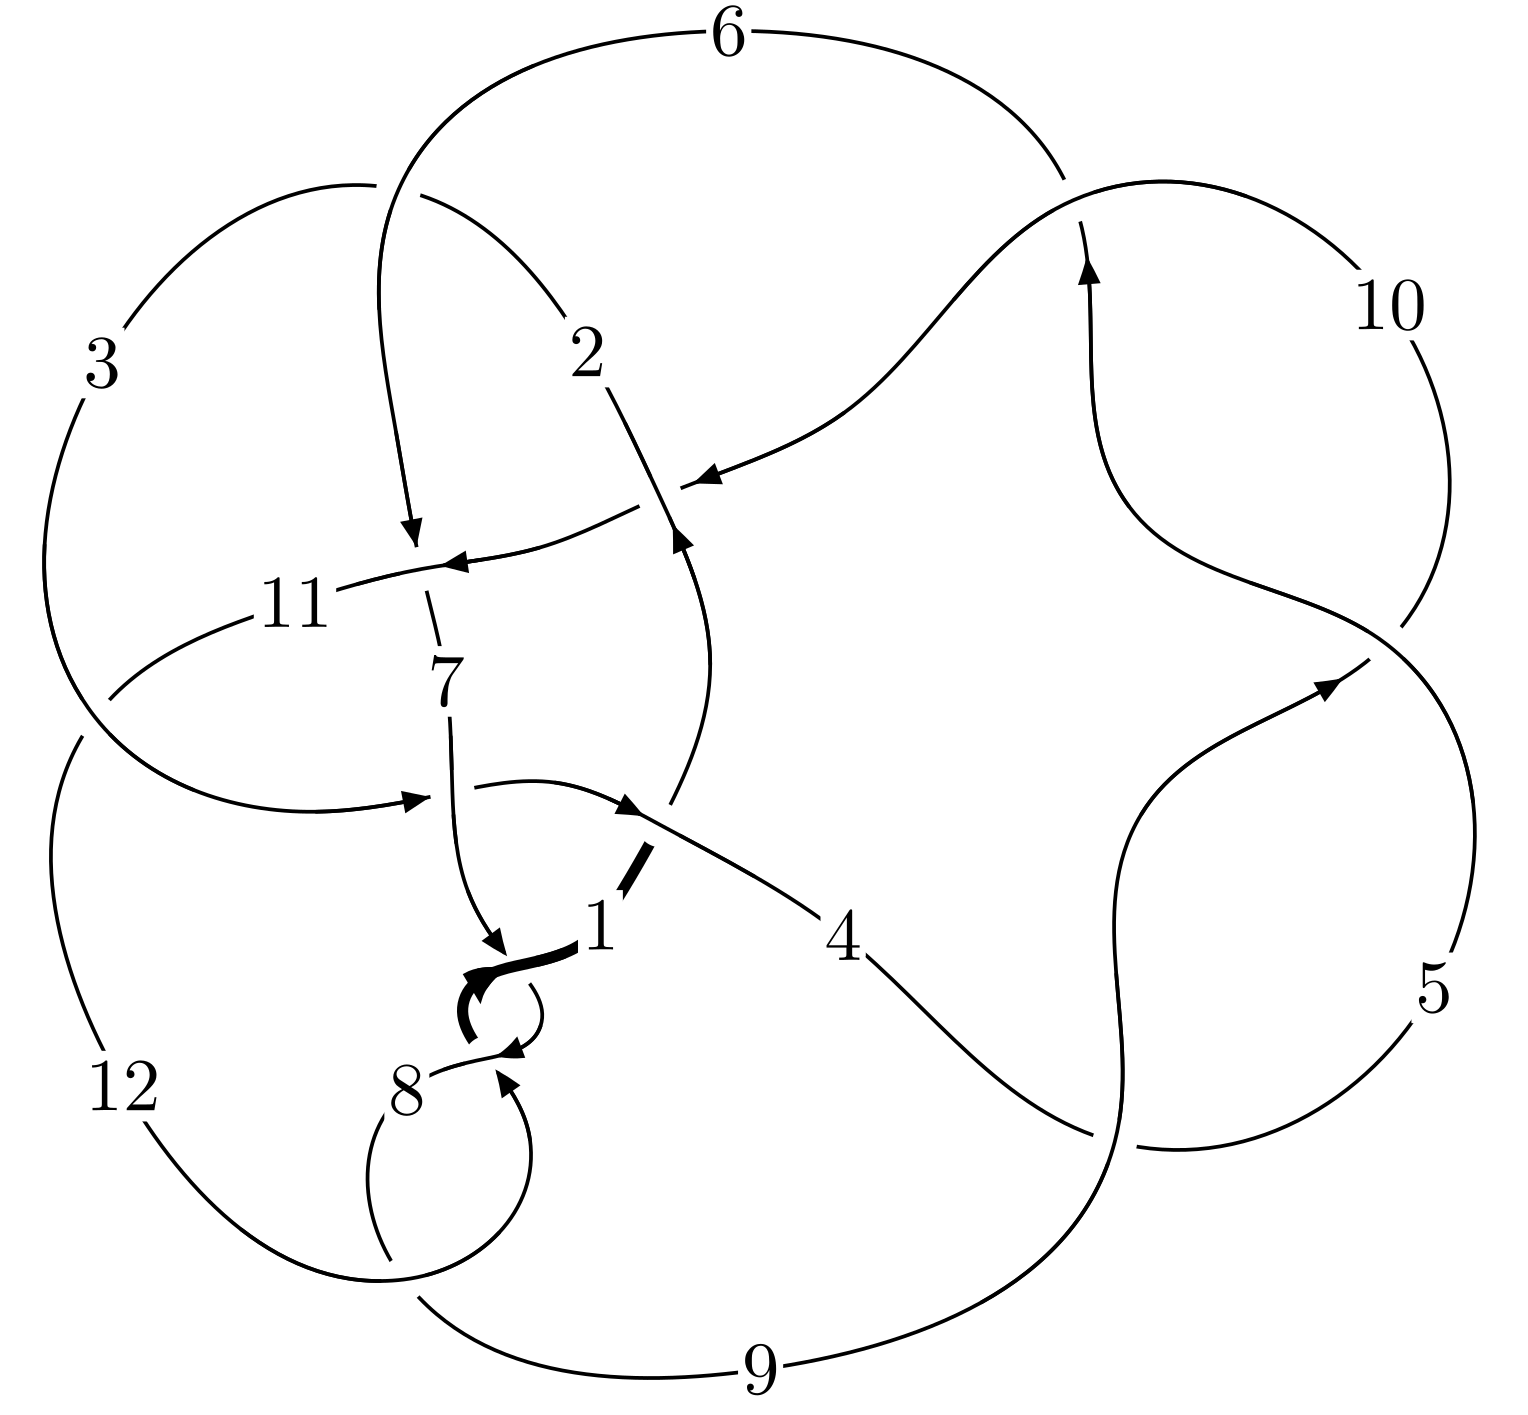
\includegraphics[width=112pt]{../../../GIT/diagram.site/Diagrams/png/1671_12a_0870.png}\\
\ \ \ A knot diagram\footnotemark}&
\allowdisplaybreaks
\textbf{Linearized knot diagam} \\
\cline{2-2}
 &
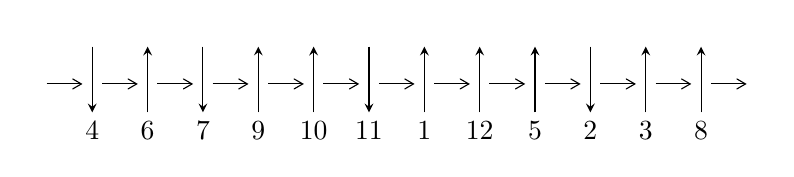
\begin{tikzpicture}[x=20pt, y=17pt]
	% nodes
	\node (C0) at (0, 0) {};
	\node (C1) at (1, 0) {};
	\node (C1U) at (1, +1) {};
	\node (C1D) at (1, -1) {4};

	\node (C2) at (2, 0) {};
	\node (C2U) at (2, +1) {};
	\node (C2D) at (2, -1) {6};

	\node (C3) at (3, 0) {};
	\node (C3U) at (3, +1) {};
	\node (C3D) at (3, -1) {7};

	\node (C4) at (4, 0) {};
	\node (C4U) at (4, +1) {};
	\node (C4D) at (4, -1) {9};

	\node (C5) at (5, 0) {};
	\node (C5U) at (5, +1) {};
	\node (C5D) at (5, -1) {10};

	\node (C6) at (6, 0) {};
	\node (C6U) at (6, +1) {};
	\node (C6D) at (6, -1) {11};

	\node (C7) at (7, 0) {};
	\node (C7U) at (7, +1) {};
	\node (C7D) at (7, -1) {1};

	\node (C8) at (8, 0) {};
	\node (C8U) at (8, +1) {};
	\node (C8D) at (8, -1) {12};

	\node (C9) at (9, 0) {};
	\node (C9U) at (9, +1) {};
	\node (C9D) at (9, -1) {5};

	\node (C10) at (10, 0) {};
	\node (C10U) at (10, +1) {};
	\node (C10D) at (10, -1) {2};

	\node (C11) at (11, 0) {};
	\node (C11U) at (11, +1) {};
	\node (C11D) at (11, -1) {3};

	\node (C12) at (12, 0) {};
	\node (C12U) at (12, +1) {};
	\node (C12D) at (12, -1) {8};
	\node (C13) at (13, 0) {};

	% arrows
	\draw[->,>={angle 60}]
	(C0) edge (C1) (C1) edge (C2) (C2) edge (C3) (C3) edge (C4) (C4) edge (C5) (C5) edge (C6) (C6) edge (C7) (C7) edge (C8) (C8) edge (C9) (C9) edge (C10) (C10) edge (C11) (C11) edge (C12) (C12) edge (C13) ;	\draw[->,>=stealth]
	(C1U) edge (C1D) (C2D) edge (C2U) (C3U) edge (C3D) (C4D) edge (C4U) (C5D) edge (C5U) (C6U) edge (C6D) (C7D) edge (C7U) (C8D) edge (C8U) (C9D) edge (C9U) (C10U) edge (C10D) (C11D) edge (C11U) (C12D) edge (C12U) ;
	\end{tikzpicture} \\
\hhline{~~} \\& 
\textbf{Solving Sequence} \\ \cline{2-2} 
 &
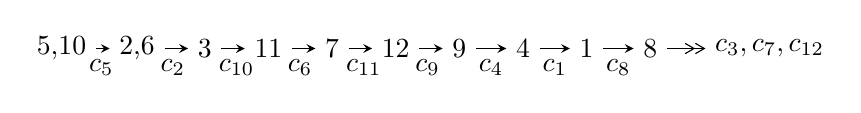
\begin{tikzpicture}[x=23pt, y=7pt]
	% node
	\node (A0) at (-1/8, 0) {5,10};
	\node (A1) at (17/16, 0) {2,6};
	\node (A2) at (17/8, 0) {3};
	\node (A3) at (25/8, 0) {11};
	\node (A4) at (33/8, 0) {7};
	\node (A5) at (41/8, 0) {12};
	\node (A6) at (49/8, 0) {9};
	\node (A7) at (57/8, 0) {4};
	\node (A8) at (65/8, 0) {1};
	\node (A9) at (73/8, 0) {8};
	\node (C1) at (1/2, -1) {$c_{5}$};
	\node (C2) at (13/8, -1) {$c_{2}$};
	\node (C3) at (21/8, -1) {$c_{10}$};
	\node (C4) at (29/8, -1) {$c_{6}$};
	\node (C5) at (37/8, -1) {$c_{11}$};
	\node (C6) at (45/8, -1) {$c_{9}$};
	\node (C7) at (53/8, -1) {$c_{4}$};
	\node (C8) at (61/8, -1) {$c_{1}$};
	\node (C9) at (69/8, -1) {$c_{8}$};
	\node (A10) at (11, 0) {$c_{3},c_{7},c_{12}$};

	% edge
	\draw[->,>=stealth]	
	(A0) edge (A1) (A1) edge (A2) (A2) edge (A3) (A3) edge (A4) (A4) edge (A5) (A5) edge (A6) (A6) edge (A7) (A7) edge (A8) (A8) edge (A9) ;
	\draw[->>,>={angle 60}]	
	(A9) edge (A10);
\end{tikzpicture} \\ 

\end{tabular} \\

\footnotetext{
The image of knot diagram is generated by the software ``\textbf{Draw programme}" developed by Andrew Bartholomew(\url{http://www.layer8.co.uk/maths/draw/index.htm\#Running-draw}), where we modified some parts for our purpose(\url{https://github.com/CATsTAILs/LinksPainter}).
}\phantom \\ \newline 
\centering \textbf{Ideals for irreducible components\footnotemark of $X_{\text{par}}$} 
 
\begin{align*}
I^u_{1}&=\langle 
-6.54960\times10^{370} u^{119}+2.86117\times10^{370} u^{118}+\cdots+1.62945\times10^{371} b-1.98484\times10^{372},\\
\phantom{I^u_{1}}&\phantom{= \langle  }-8.95643\times10^{372} u^{119}+1.63636\times10^{373} u^{118}+\cdots+1.62945\times10^{371} a-6.28178\times10^{373},\\
\phantom{I^u_{1}}&\phantom{= \langle  }u^{120}-2 u^{119}+\cdots+39 u-1\rangle \\
I^u_{2}&=\langle 
876 u^{26}+1025 u^{25}+\cdots+2461 b-1161,\;- u^{23}+u^{22}+\cdots+a+5,\;u^{27}- u^{26}+\cdots+10 u^2+1\rangle \\
\\
\end{align*}
\raggedright * 2 irreducible components of $\dim_{\mathbb{C}}=0$, with total 147 representations.\\
\footnotetext{All coefficients of polynomials are rational numbers. But the coefficients are sometimes approximated in decimal forms when there is not enough margin.}
\newpage
\renewcommand{\arraystretch}{1}
\centering \section*{I. $I^u_{1}= \langle -6.55\times10^{370} u^{119}+2.86\times10^{370} u^{118}+\cdots+1.63\times10^{371} b-1.98\times10^{372},\;-8.96\times10^{372} u^{119}+1.64\times10^{373} u^{118}+\cdots+1.63\times10^{371} a-6.28\times10^{373},\;u^{120}-2 u^{119}+\cdots+39 u-1 \rangle$}
\flushleft \textbf{(i) Arc colorings}\\
\begin{tabular}{m{7pt} m{180pt} m{7pt} m{180pt} }
\flushright $a_{5}=$&$\begin{pmatrix}1\\0\end{pmatrix}$ \\
\flushright $a_{10}=$&$\begin{pmatrix}0\\u\end{pmatrix}$ \\
\flushright $a_{2}=$&$\begin{pmatrix}54.9659 u^{119}-100.424 u^{118}+\cdots-11615.5 u+385.515\\0.401951 u^{119}-0.175591 u^{118}+\cdots-227.860 u+12.1810\end{pmatrix}$ \\
\flushright $a_{6}=$&$\begin{pmatrix}1\\- u^2\end{pmatrix}$ \\
\flushright $a_{3}=$&$\begin{pmatrix}56.8121 u^{119}-104.056 u^{118}+\cdots-12159.2 u+407.204\\0.590180 u^{119}-0.157202 u^{118}+\cdots-227.338 u+12.1203\end{pmatrix}$ \\
\flushright $a_{11}=$&$\begin{pmatrix}33.1201 u^{119}-60.7925 u^{118}+\cdots-7301.06 u+249.734\\2.18895 u^{119}-3.76307 u^{118}+\cdots-16.5883 u-3.37165\end{pmatrix}$ \\
\flushright $a_{7}=$&$\begin{pmatrix}51.0385 u^{119}-90.7444 u^{118}+\cdots-8238.29 u+256.337\\-1.20417 u^{119}+2.82829 u^{118}+\cdots+732.655 u-28.8332\end{pmatrix}$ \\
\flushright $a_{12}=$&$\begin{pmatrix}19.8253 u^{119}-40.2460 u^{118}+\cdots-9327.21 u+368.069\\2.65349 u^{119}-4.92166 u^{118}+\cdots-696.236 u+27.8624\end{pmatrix}$ \\
\flushright $a_{9}=$&$\begin{pmatrix}- u\\u\end{pmatrix}$ \\
\flushright $a_{4}=$&$\begin{pmatrix}- u^2+1\\u^2\end{pmatrix}$ \\
\flushright $a_{1}=$&$\begin{pmatrix}52.8259 u^{119}-96.9718 u^{118}+\cdots-11517.1 u+387.963\\0.515629 u^{119}+0.0216045 u^{118}+\cdots-214.156 u+11.7777\end{pmatrix}$ \\
\flushright $a_{8}=$&$\begin{pmatrix}25.1563 u^{119}-44.6996 u^{118}+\cdots-5453.41 u+212.193\\-6.89765 u^{119}+12.3493 u^{118}+\cdots+2103.98 u-78.2389\end{pmatrix}$\\&\end{tabular}
\flushleft \textbf{(ii) Obstruction class $= -1$}\\~\\
\flushleft \textbf{(iii) Cusp Shapes $= 40.6118 u^{119}-72.5190 u^{118}+\cdots-6607.82 u+200.568$}\\~\\
\newpage\renewcommand{\arraystretch}{1}
\flushleft \textbf{(iv) u-Polynomials at the component}\newline \\
\begin{tabular}{m{50pt}|m{274pt}}
Crossings & \hspace{64pt}u-Polynomials at each crossing \\
\hline $$\begin{aligned}c_{1}\end{aligned}$$&$\begin{aligned}
&u^{120}+2 u^{119}+\cdots-340978 u+22627
\end{aligned}$\\
\hline $$\begin{aligned}c_{2}\end{aligned}$$&$\begin{aligned}
&u^{120}-3 u^{119}+\cdots+52767 u+9067
\end{aligned}$\\
\hline $$\begin{aligned}c_{3}\end{aligned}$$&$\begin{aligned}
&u^{120}-5 u^{119}+\cdots-58768 u+18208
\end{aligned}$\\
\hline $$\begin{aligned}c_{4},c_{5},c_{9}\end{aligned}$$&$\begin{aligned}
&u^{120}+2 u^{119}+\cdots-39 u-1
\end{aligned}$\\
\hline $$\begin{aligned}c_{6}\end{aligned}$$&$\begin{aligned}
&u^{120}-11 u^{118}+\cdots+29 u+1
\end{aligned}$\\
\hline $$\begin{aligned}c_{7},c_{8},c_{12}\end{aligned}$$&$\begin{aligned}
&u^{120}+57 u^{118}+\cdots+179 u+43
\end{aligned}$\\
\hline $$\begin{aligned}c_{10}\end{aligned}$$&$\begin{aligned}
&u^{120}+3 u^{119}+\cdots+1582 u+527
\end{aligned}$\\
\hline $$\begin{aligned}c_{11}\end{aligned}$$&$\begin{aligned}
&u^{120}+3 u^{119}+\cdots+4239 u-3181
\end{aligned}$\\
\hline
\end{tabular}\\~\\
\newpage\renewcommand{\arraystretch}{1}
\flushleft \textbf{(v) Riley Polynomials at the component}\newline \\
\begin{tabular}{m{50pt}|m{274pt}}
Crossings & \hspace{64pt}Riley Polynomials at each crossing \\
\hline $$\begin{aligned}c_{1}\end{aligned}$$&$\begin{aligned}
&y^{120}-12 y^{119}+\cdots-60610138314 y+511981129
\end{aligned}$\\
\hline $$\begin{aligned}c_{2}\end{aligned}$$&$\begin{aligned}
&y^{120}-37 y^{119}+\cdots-4553618133 y+82210489
\end{aligned}$\\
\hline $$\begin{aligned}c_{3}\end{aligned}$$&$\begin{aligned}
&y^{120}-45 y^{119}+\cdots-6327045888 y+331531264
\end{aligned}$\\
\hline $$\begin{aligned}c_{4},c_{5},c_{9}\end{aligned}$$&$\begin{aligned}
&y^{120}-128 y^{119}+\cdots-367 y+1
\end{aligned}$\\
\hline $$\begin{aligned}c_{6}\end{aligned}$$&$\begin{aligned}
&y^{120}-22 y^{119}+\cdots-537 y+1
\end{aligned}$\\
\hline $$\begin{aligned}c_{7},c_{8},c_{12}\end{aligned}$$&$\begin{aligned}
&y^{120}+114 y^{119}+\cdots-102991 y+1849
\end{aligned}$\\
\hline $$\begin{aligned}c_{10}\end{aligned}$$&$\begin{aligned}
&y^{120}+31 y^{119}+\cdots+2355162 y+277729
\end{aligned}$\\
\hline $$\begin{aligned}c_{11}\end{aligned}$$&$\begin{aligned}
&y^{120}-3 y^{119}+\cdots-363476617 y+10118761
\end{aligned}$\\
\hline
\end{tabular}\\~\\
\newpage\flushleft \textbf{(vi) Complex Volumes and Cusp Shapes}
$$\begin{array}{c|c|c}  
\text{Solutions to }I^u_{1}& \I (\text{vol} + \sqrt{-1}CS) & \text{Cusp shape}\\
 \hline 
\begin{aligned}
u &= \phantom{-}0.478483 + 0.849417 I \\
a &= -0.767371 + 0.191220 I \\
b &= \phantom{-}0.550456 + 0.091495 I\end{aligned}
 & -0.61287 - 4.48013 I & \phantom{-0.000000 } 0 \\ \hline\begin{aligned}
u &= \phantom{-}0.478483 - 0.849417 I \\
a &= -0.767371 - 0.191220 I \\
b &= \phantom{-}0.550456 - 0.091495 I\end{aligned}
 & -0.61287 + 4.48013 I & \phantom{-0.000000 } 0 \\ \hline\begin{aligned}
u &= \phantom{-}0.575507 + 0.779779 I \\
a &= \phantom{-}0.173619 + 1.369450 I \\
b &= \phantom{-}0.216728 - 0.600397 I\end{aligned}
 & -0.33148 + 9.79234 I & \phantom{-0.000000 } 0 \\ \hline\begin{aligned}
u &= \phantom{-}0.575507 - 0.779779 I \\
a &= \phantom{-}0.173619 - 1.369450 I \\
b &= \phantom{-}0.216728 + 0.600397 I\end{aligned}
 & -0.33148 - 9.79234 I & \phantom{-0.000000 } 0 \\ \hline\begin{aligned}
u &= \phantom{-}0.273232 + 1.032380 I \\
a &= -0.463078 - 0.662791 I \\
b &= \phantom{-}0.075684 + 0.394031 I\end{aligned}
 & -1.98811 + 4.42294 I & \phantom{-0.000000 } 0 \\ \hline\begin{aligned}
u &= \phantom{-}0.273232 - 1.032380 I \\
a &= -0.463078 + 0.662791 I \\
b &= \phantom{-}0.075684 - 0.394031 I\end{aligned}
 & -1.98811 - 4.42294 I & \phantom{-0.000000 } 0 \\ \hline\begin{aligned}
u &= -0.518844 + 0.733055 I \\
a &= -0.269808 + 0.947950 I \\
b &= \phantom{-}0.123018 - 0.706042 I\end{aligned}
 & \phantom{-}1.76059 - 2.74032 I & \phantom{-0.000000 } 0 \\ \hline\begin{aligned}
u &= -0.518844 - 0.733055 I \\
a &= -0.269808 - 0.947950 I \\
b &= \phantom{-}0.123018 + 0.706042 I\end{aligned}
 & \phantom{-}1.76059 + 2.74032 I & \phantom{-0.000000 } 0 \\ \hline\begin{aligned}
u &= -0.622693 + 0.911978 I \\
a &= \phantom{-}0.189781 - 1.191170 I \\
b &= \phantom{-}0.382272 + 0.610684 I\end{aligned}
 & -6.5229 - 13.5895 I & \phantom{-0.000000 } 0 \\ \hline\begin{aligned}
u &= -0.622693 - 0.911978 I \\
a &= \phantom{-}0.189781 + 1.191170 I \\
b &= \phantom{-}0.382272 - 0.610684 I\end{aligned}
 & -6.5229 + 13.5895 I & \phantom{-0.000000 } 0\\
 \hline 
 \end{array}$$\newpage$$\begin{array}{c|c|c}  
\text{Solutions to }I^u_{1}& \I (\text{vol} + \sqrt{-1}CS) & \text{Cusp shape}\\
 \hline 
\begin{aligned}
u &= -0.753947 + 0.480130 I \\
a &= -0.780125 + 0.120594 I \\
b &= \phantom{-}0.966255 - 0.233013 I\end{aligned}
 & \phantom{-}0.000609 + 0.829262 I & \phantom{-0.000000 } 0 \\ \hline\begin{aligned}
u &= -0.753947 - 0.480130 I \\
a &= -0.780125 - 0.120594 I \\
b &= \phantom{-}0.966255 + 0.233013 I\end{aligned}
 & \phantom{-}0.000609 - 0.829262 I & \phantom{-0.000000 } 0 \\ \hline\begin{aligned}
u &= \phantom{-}0.909026 + 0.665065 I \\
a &= -0.003551 - 0.751036 I \\
b &= \phantom{-}0.040568 + 0.950919 I\end{aligned}
 & -2.61930 + 1.01094 I & \phantom{-0.000000 } 0 \\ \hline\begin{aligned}
u &= \phantom{-}0.909026 - 0.665065 I \\
a &= -0.003551 + 0.751036 I \\
b &= \phantom{-}0.040568 - 0.950919 I\end{aligned}
 & -2.61930 - 1.01094 I & \phantom{-0.000000 } 0 \\ \hline\begin{aligned}
u &= \phantom{-}1.079280 + 0.343096 I \\
a &= \phantom{-}0.866867 - 0.135791 I \\
b &= \phantom{-}0.558626 - 0.074170 I\end{aligned}
 & -4.49341 - 2.35363 I & \phantom{-0.000000 } 0 \\ \hline\begin{aligned}
u &= \phantom{-}1.079280 - 0.343096 I \\
a &= \phantom{-}0.866867 + 0.135791 I \\
b &= \phantom{-}0.558626 + 0.074170 I\end{aligned}
 & -4.49341 + 2.35363 I & \phantom{-0.000000 } 0 \\ \hline\begin{aligned}
u &= -0.708210 + 0.478105 I \\
a &= \phantom{-}1.41992 + 0.30534 I \\
b &= -0.673792 + 0.470912 I\end{aligned}
 & -7.25207 + 0.98951 I & \phantom{-0.000000 } 0 \\ \hline\begin{aligned}
u &= -0.708210 - 0.478105 I \\
a &= \phantom{-}1.41992 - 0.30534 I \\
b &= -0.673792 - 0.470912 I\end{aligned}
 & -7.25207 - 0.98951 I & \phantom{-0.000000 } 0 \\ \hline\begin{aligned}
u &= -0.830894 + 0.185761 I \\
a &= \phantom{-}1.169230 + 0.325097 I \\
b &= \phantom{-}0.248193 - 0.143424 I\end{aligned}
 & \phantom{-}0.246168 + 0.061672 I & \phantom{-0.000000 } 0 \\ \hline\begin{aligned}
u &= -0.830894 - 0.185761 I \\
a &= \phantom{-}1.169230 - 0.325097 I \\
b &= \phantom{-}0.248193 + 0.143424 I\end{aligned}
 & \phantom{-}0.246168 - 0.061672 I & \phantom{-0.000000 } 0\\
 \hline 
 \end{array}$$\newpage$$\begin{array}{c|c|c}  
\text{Solutions to }I^u_{1}& \I (\text{vol} + \sqrt{-1}CS) & \text{Cusp shape}\\
 \hline 
\begin{aligned}
u &= \phantom{-}0.452519 + 1.057460 I \\
a &= \phantom{-}0.553440 + 0.331900 I \\
b &= \phantom{-}0.126470 - 0.168338 I\end{aligned}
 & -4.38678 + 5.06586 I & \phantom{-0.000000 } 0 \\ \hline\begin{aligned}
u &= \phantom{-}0.452519 - 1.057460 I \\
a &= \phantom{-}0.553440 - 0.331900 I \\
b &= \phantom{-}0.126470 + 0.168338 I\end{aligned}
 & -4.38678 - 5.06586 I & \phantom{-0.000000 } 0 \\ \hline\begin{aligned}
u &= \phantom{-}1.149860 + 0.070091 I \\
a &= -0.006453 + 0.395205 I \\
b &= \phantom{-}1.15683 - 1.55091 I\end{aligned}
 & -3.75681 - 1.03419 I & \phantom{-0.000000 } 0 \\ \hline\begin{aligned}
u &= \phantom{-}1.149860 - 0.070091 I \\
a &= -0.006453 - 0.395205 I \\
b &= \phantom{-}1.15683 + 1.55091 I\end{aligned}
 & -3.75681 + 1.03419 I & \phantom{-0.000000 } 0 \\ \hline\begin{aligned}
u &= \phantom{-}0.151147 + 0.823040 I \\
a &= \phantom{-}0.86443 + 1.24866 I \\
b &= \phantom{-}0.146533 - 0.137851 I\end{aligned}
 & -8.39973 + 2.22044 I & \phantom{-0.000000 } 0 \\ \hline\begin{aligned}
u &= \phantom{-}0.151147 - 0.823040 I \\
a &= \phantom{-}0.86443 - 1.24866 I \\
b &= \phantom{-}0.146533 + 0.137851 I\end{aligned}
 & -8.39973 - 2.22044 I & \phantom{-0.000000 } 0 \\ \hline\begin{aligned}
u &= -0.422357 + 0.704219 I \\
a &= \phantom{-}0.820403 - 0.635098 I \\
b &= -0.023246 + 0.188752 I\end{aligned}
 & \phantom{-}1.69314 - 1.85272 I & \phantom{-0.000000 } 0 \\ \hline\begin{aligned}
u &= -0.422357 - 0.704219 I \\
a &= \phantom{-}0.820403 + 0.635098 I \\
b &= -0.023246 - 0.188752 I\end{aligned}
 & \phantom{-}1.69314 + 1.85272 I & \phantom{-0.000000 } 0 \\ \hline\begin{aligned}
u &= -0.403079 + 0.670090 I \\
a &= \phantom{-}0.41244 - 1.67380 I \\
b &= \phantom{-}0.048249 + 0.433133 I\end{aligned}
 & -1.01899 - 4.94043 I & \phantom{-0.000000 } 0 \\ \hline\begin{aligned}
u &= -0.403079 - 0.670090 I \\
a &= \phantom{-}0.41244 + 1.67380 I \\
b &= \phantom{-}0.048249 - 0.433133 I\end{aligned}
 & -1.01899 + 4.94043 I & \phantom{-0.000000 } 0\\
 \hline 
 \end{array}$$\newpage$$\begin{array}{c|c|c}  
\text{Solutions to }I^u_{1}& \I (\text{vol} + \sqrt{-1}CS) & \text{Cusp shape}\\
 \hline 
\begin{aligned}
u &= -0.608246 + 1.086410 I \\
a &= -0.612090 - 0.173967 I \\
b &= \phantom{-}0.405539 - 0.264911 I\end{aligned}
 & -6.72107 + 7.19768 I & \phantom{-0.000000 } 0 \\ \hline\begin{aligned}
u &= -0.608246 - 1.086410 I \\
a &= -0.612090 + 0.173967 I \\
b &= \phantom{-}0.405539 + 0.264911 I\end{aligned}
 & -6.72107 - 7.19768 I & \phantom{-0.000000 } 0 \\ \hline\begin{aligned}
u &= \phantom{-}1.089660 + 0.606849 I \\
a &= -0.618763 - 0.132814 I \\
b &= \phantom{-}0.876160 + 0.605218 I\end{aligned}
 & -5.69944 + 2.78171 I & \phantom{-0.000000 } 0 \\ \hline\begin{aligned}
u &= \phantom{-}1.089660 - 0.606849 I \\
a &= -0.618763 + 0.132814 I \\
b &= \phantom{-}0.876160 - 0.605218 I\end{aligned}
 & -5.69944 - 2.78171 I & \phantom{-0.000000 } 0 \\ \hline\begin{aligned}
u &= -0.726933 + 0.067830 I \\
a &= \phantom{-}0.42675 + 1.56256 I \\
b &= \phantom{-}0.50877 - 1.86490 I\end{aligned}
 & -4.06221 - 5.35034 I & \phantom{-0.000000 } 0 \\ \hline\begin{aligned}
u &= -0.726933 - 0.067830 I \\
a &= \phantom{-}0.42675 - 1.56256 I \\
b &= \phantom{-}0.50877 + 1.86490 I\end{aligned}
 & -4.06221 + 5.35034 I & \phantom{-0.000000 } 0 \\ \hline\begin{aligned}
u &= -0.405015 + 0.588736 I \\
a &= -0.35512 + 1.98421 I \\
b &= -0.710110 - 0.653830 I\end{aligned}
 & -8.09284 - 4.73305 I & \phantom{-0.000000 } 0 \\ \hline\begin{aligned}
u &= -0.405015 - 0.588736 I \\
a &= -0.35512 - 1.98421 I \\
b &= -0.710110 + 0.653830 I\end{aligned}
 & -8.09284 + 4.73305 I & \phantom{-0.000000 } 0 \\ \hline\begin{aligned}
u &= \phantom{-}0.547603 + 0.454014 I \\
a &= \phantom{-}0.585941 - 0.526840 I \\
b &= \phantom{-}0.159576 + 0.709440 I\end{aligned}
 & -2.85217 + 1.79301 I & \phantom{-0.000000 } 0 \\ \hline\begin{aligned}
u &= \phantom{-}0.547603 - 0.454014 I \\
a &= \phantom{-}0.585941 + 0.526840 I \\
b &= \phantom{-}0.159576 - 0.709440 I\end{aligned}
 & -2.85217 - 1.79301 I & \phantom{-0.000000 } 0\\
 \hline 
 \end{array}$$\newpage$$\begin{array}{c|c|c}  
\text{Solutions to }I^u_{1}& \I (\text{vol} + \sqrt{-1}CS) & \text{Cusp shape}\\
 \hline 
\begin{aligned}
u &= -1.287130 + 0.226241 I \\
a &= \phantom{-}0.453160 + 1.250730 I \\
b &= -0.52610 - 2.67215 I\end{aligned}
 & -3.99178 - 5.99598 I & \phantom{-0.000000 } 0 \\ \hline\begin{aligned}
u &= -1.287130 - 0.226241 I \\
a &= \phantom{-}0.453160 - 1.250730 I \\
b &= -0.52610 + 2.67215 I\end{aligned}
 & -3.99178 + 5.99598 I & \phantom{-0.000000 } 0 \\ \hline\begin{aligned}
u &= \phantom{-}0.508195 + 0.415399 I \\
a &= \phantom{-}0.48567 - 1.88483 I \\
b &= -0.297989 + 0.609389 I\end{aligned}
 & -1.49358 + 2.77561 I & \phantom{-0.000000 } 0 \\ \hline\begin{aligned}
u &= \phantom{-}0.508195 - 0.415399 I \\
a &= \phantom{-}0.48567 + 1.88483 I \\
b &= -0.297989 - 0.609389 I\end{aligned}
 & -1.49358 - 2.77561 I & \phantom{-0.000000 } 0 \\ \hline\begin{aligned}
u &= \phantom{-}0.162960 + 0.630383 I \\
a &= \phantom{-}0.103205 - 0.977469 I \\
b &= -1.04484 + 0.96767 I\end{aligned}
 & -7.25062 + 5.95071 I & \phantom{-0.000000 } 0 \\ \hline\begin{aligned}
u &= \phantom{-}0.162960 - 0.630383 I \\
a &= \phantom{-}0.103205 + 0.977469 I \\
b &= -1.04484 - 0.96767 I\end{aligned}
 & -7.25062 - 5.95071 I & \phantom{-0.000000 } 0 \\ \hline\begin{aligned}
u &= -1.358730 + 0.031900 I \\
a &= -0.128589 - 0.355133 I \\
b &= \phantom{-}0.68025 + 1.82260 I\end{aligned}
 & \phantom{-}2.80943 - 1.19492 I & \phantom{-0.000000 } 0 \\ \hline\begin{aligned}
u &= -1.358730 - 0.031900 I \\
a &= -0.128589 + 0.355133 I \\
b &= \phantom{-}0.68025 - 1.82260 I\end{aligned}
 & \phantom{-}2.80943 + 1.19492 I & \phantom{-0.000000 } 0 \\ \hline\begin{aligned}
u &= \phantom{-}1.38527\phantom{ +0.000000I} \\
a &= \phantom{-}1.05701\phantom{ +0.000000I} \\
b &= -0.374028\phantom{ +0.000000I}\end{aligned}
 & \phantom{-}2.28263\phantom{ +0.000000I} & \phantom{-0.000000 } 0 \\ \hline\begin{aligned}
u &= \phantom{-}1.396410 + 0.007950 I \\
a &= -0.577667 + 0.692521 I \\
b &= -0.48919 - 2.39754 I\end{aligned}
 & \phantom{-}2.80753 + 2.62829 I & \phantom{-0.000000 } 0\\
 \hline 
 \end{array}$$\newpage$$\begin{array}{c|c|c}  
\text{Solutions to }I^u_{1}& \I (\text{vol} + \sqrt{-1}CS) & \text{Cusp shape}\\
 \hline 
\begin{aligned}
u &= \phantom{-}1.396410 - 0.007950 I \\
a &= -0.577667 - 0.692521 I \\
b &= -0.48919 + 2.39754 I\end{aligned}
 & \phantom{-}2.80753 - 2.62829 I & \phantom{-0.000000 } 0 \\ \hline\begin{aligned}
u &= \phantom{-}1.402730 + 0.038408 I \\
a &= \phantom{-}0.63374 - 1.48215 I \\
b &= -0.66816 + 3.36307 I\end{aligned}
 & \phantom{-}5.44161 + 3.32832 I & \phantom{-0.000000 } 0 \\ \hline\begin{aligned}
u &= \phantom{-}1.402730 - 0.038408 I \\
a &= \phantom{-}0.63374 + 1.48215 I \\
b &= -0.66816 - 3.36307 I\end{aligned}
 & \phantom{-}5.44161 - 3.32832 I & \phantom{-0.000000 } 0 \\ \hline\begin{aligned}
u &= -1.406160 + 0.099173 I \\
a &= \phantom{-}1.014220 - 0.092722 I \\
b &= -0.270731 + 0.472154 I\end{aligned}
 & -1.96529 - 4.26450 I & \phantom{-0.000000 } 0 \\ \hline\begin{aligned}
u &= -1.406160 - 0.099173 I \\
a &= \phantom{-}1.014220 + 0.092722 I \\
b &= -0.270731 - 0.472154 I\end{aligned}
 & -1.96529 + 4.26450 I & \phantom{-0.000000 } 0 \\ \hline\begin{aligned}
u &= \phantom{-}1.404700 + 0.130601 I \\
a &= -0.108113 + 0.283629 I \\
b &= \phantom{-}0.58648 - 2.23100 I\end{aligned}
 & \phantom{-}3.59810 + 5.30904 I & \phantom{-0.000000 } 0 \\ \hline\begin{aligned}
u &= \phantom{-}1.404700 - 0.130601 I \\
a &= -0.108113 - 0.283629 I \\
b &= \phantom{-}0.58648 + 2.23100 I\end{aligned}
 & \phantom{-}3.59810 - 5.30904 I & \phantom{-0.000000 } 0 \\ \hline\begin{aligned}
u &= -1.401130 + 0.190037 I \\
a &= -0.079236 - 0.260877 I \\
b &= \phantom{-}0.72768 + 2.52738 I\end{aligned}
 & -2.21911 - 8.79214 I & \phantom{-0.000000 } 0 \\ \hline\begin{aligned}
u &= -1.401130 - 0.190037 I \\
a &= -0.079236 + 0.260877 I \\
b &= \phantom{-}0.72768 - 2.52738 I\end{aligned}
 & -2.21911 + 8.79214 I & \phantom{-0.000000 } 0 \\ \hline\begin{aligned}
u &= -0.223950 + 0.539425 I \\
a &= \phantom{-}0.376489 + 1.062640 I \\
b &= -0.784184 - 0.764176 I\end{aligned}
 & -1.58940 - 3.03839 I & \phantom{-0.000000 -}0. + 8.59848 I\\
 \hline 
 \end{array}$$\newpage$$\begin{array}{c|c|c}  
\text{Solutions to }I^u_{1}& \I (\text{vol} + \sqrt{-1}CS) & \text{Cusp shape}\\
 \hline 
\begin{aligned}
u &= -0.223950 - 0.539425 I \\
a &= \phantom{-}0.376489 - 1.062640 I \\
b &= -0.784184 + 0.764176 I\end{aligned}
 & -1.58940 + 3.03839 I & \phantom{-0.000000 } 0. - 8.59848 I \\ \hline\begin{aligned}
u &= -1.42603 + 0.04080 I \\
a &= -0.538009 + 0.495308 I \\
b &= -0.009278 - 1.061150 I\end{aligned}
 & \phantom{-}3.54135 - 2.83450 I & \phantom{-0.000000 } 0 \\ \hline\begin{aligned}
u &= -1.42603 - 0.04080 I \\
a &= -0.538009 - 0.495308 I \\
b &= -0.009278 + 1.061150 I\end{aligned}
 & \phantom{-}3.54135 + 2.83450 I & \phantom{-0.000000 } 0 \\ \hline\begin{aligned}
u &= -1.41717 + 0.23454 I \\
a &= -0.125846 + 0.883347 I \\
b &= \phantom{-}0.48427 - 2.14137 I\end{aligned}
 & \phantom{-}5.82758 - 0.12145 I & \phantom{-0.000000 } 0 \\ \hline\begin{aligned}
u &= -1.41717 - 0.23454 I \\
a &= -0.125846 - 0.883347 I \\
b &= \phantom{-}0.48427 + 2.14137 I\end{aligned}
 & \phantom{-}5.82758 + 0.12145 I & \phantom{-0.000000 } 0 \\ \hline\begin{aligned}
u &= -1.44781 + 0.02957 I \\
a &= \phantom{-}0.85478 - 1.42201 I \\
b &= -1.06793 + 3.33256 I\end{aligned}
 & \phantom{-}6.68138 - 3.02805 I & \phantom{-0.000000 } 0 \\ \hline\begin{aligned}
u &= -1.44781 - 0.02957 I \\
a &= \phantom{-}0.85478 + 1.42201 I \\
b &= -1.06793 - 3.33256 I\end{aligned}
 & \phantom{-}6.68138 + 3.02805 I & \phantom{-0.000000 } 0 \\ \hline\begin{aligned}
u &= \phantom{-}1.45894 + 0.10853 I \\
a &= \phantom{-}1.13982 + 1.10887 I \\
b &= -1.51407 - 2.79596 I\end{aligned}
 & \phantom{-}0.31268 + 8.12438 I & \phantom{-0.000000 } 0 \\ \hline\begin{aligned}
u &= \phantom{-}1.45894 - 0.10853 I \\
a &= \phantom{-}1.13982 - 1.10887 I \\
b &= -1.51407 + 2.79596 I\end{aligned}
 & \phantom{-}0.31268 - 8.12438 I & \phantom{-0.000000 } 0 \\ \hline\begin{aligned}
u &= -0.514478\phantom{ +0.000000I} \\
a &= \phantom{-}0.541958\phantom{ +0.000000I} \\
b &= \phantom{-}0.362022\phantom{ +0.000000I}\end{aligned}
 & \phantom{-}0.861482\phantom{ +0.000000I} & \phantom{-}11.4300\phantom{ +0.000000I}\\
 \hline 
 \end{array}$$\newpage$$\begin{array}{c|c|c}  
\text{Solutions to }I^u_{1}& \I (\text{vol} + \sqrt{-1}CS) & \text{Cusp shape}\\
 \hline 
\begin{aligned}
u &= -1.49675 + 0.06976 I \\
a &= -0.520851 - 0.716080 I \\
b &= -0.14152 + 2.61330 I\end{aligned}
 & \phantom{-}7.58116 - 4.68582 I & \phantom{-0.000000 } 0 \\ \hline\begin{aligned}
u &= -1.49675 - 0.06976 I \\
a &= -0.520851 + 0.716080 I \\
b &= -0.14152 - 2.61330 I\end{aligned}
 & \phantom{-}7.58116 + 4.68582 I & \phantom{-0.000000 } 0 \\ \hline\begin{aligned}
u &= \phantom{-}1.48951 + 0.18039 I \\
a &= -0.361848 + 1.163260 I \\
b &= \phantom{-}1.02518 - 3.44855 I\end{aligned}
 & -1.86405 + 7.47025 I & \phantom{-0.000000 } 0 \\ \hline\begin{aligned}
u &= \phantom{-}1.48951 - 0.18039 I \\
a &= -0.361848 - 1.163260 I \\
b &= \phantom{-}1.02518 + 3.44855 I\end{aligned}
 & -1.86405 - 7.47025 I & \phantom{-0.000000 } 0 \\ \hline\begin{aligned}
u &= \phantom{-}1.48920 + 0.22925 I \\
a &= \phantom{-}0.630966 - 1.058700 I \\
b &= -0.87163 + 2.67400 I\end{aligned}
 & \phantom{-}5.17663 + 8.19160 I & \phantom{-0.000000 } 0 \\ \hline\begin{aligned}
u &= \phantom{-}1.48920 - 0.22925 I \\
a &= \phantom{-}0.630966 + 1.058700 I \\
b &= -0.87163 - 2.67400 I\end{aligned}
 & \phantom{-}5.17663 - 8.19160 I & \phantom{-0.000000 } 0 \\ \hline\begin{aligned}
u &= -1.47417 + 0.34800 I \\
a &= -0.462583 - 0.762589 I \\
b &= \phantom{-}0.23733 + 1.95877 I\end{aligned}
 & \phantom{-}3.69434 - 9.18982 I & \phantom{-0.000000 } 0 \\ \hline\begin{aligned}
u &= -1.47417 - 0.34800 I \\
a &= -0.462583 + 0.762589 I \\
b &= \phantom{-}0.23733 - 1.95877 I\end{aligned}
 & \phantom{-}3.69434 + 9.18982 I & \phantom{-0.000000 } 0 \\ \hline\begin{aligned}
u &= -1.52450 + 0.10022 I \\
a &= -0.792506 - 1.004320 I \\
b &= \phantom{-}1.45076 + 2.76776 I\end{aligned}
 & \phantom{-}5.30025 - 4.55141 I & \phantom{-0.000000 } 0 \\ \hline\begin{aligned}
u &= -1.52450 - 0.10022 I \\
a &= -0.792506 + 1.004320 I \\
b &= \phantom{-}1.45076 - 2.76776 I\end{aligned}
 & \phantom{-}5.30025 + 4.55141 I & \phantom{-0.000000 } 0\\
 \hline 
 \end{array}$$\newpage$$\begin{array}{c|c|c}  
\text{Solutions to }I^u_{1}& \I (\text{vol} + \sqrt{-1}CS) & \text{Cusp shape}\\
 \hline 
\begin{aligned}
u &= \phantom{-}1.53217\phantom{ +0.000000I} \\
a &= -1.18540\phantom{ +0.000000I} \\
b &= \phantom{-}1.96526\phantom{ +0.000000I}\end{aligned}
 & \phantom{-}7.64836\phantom{ +0.000000I} & \phantom{-0.000000 } 0 \\ \hline\begin{aligned}
u &= \phantom{-}1.53210 + 0.02964 I \\
a &= -0.479060 + 0.317483 I \\
b &= \phantom{-}0.124509 - 0.884896 I\end{aligned}
 & \phantom{-}7.86979 + 0.12335 I & \phantom{-0.000000 } 0 \\ \hline\begin{aligned}
u &= \phantom{-}1.53210 - 0.02964 I \\
a &= -0.479060 - 0.317483 I \\
b &= \phantom{-}0.124509 + 0.884896 I\end{aligned}
 & \phantom{-}7.86979 - 0.12335 I & \phantom{-0.000000 } 0 \\ \hline\begin{aligned}
u &= \phantom{-}1.50554 + 0.28596 I \\
a &= \phantom{-}0.061157 - 0.855092 I \\
b &= \phantom{-}0.05022 + 2.13935 I\end{aligned}
 & \phantom{-}7.92931 + 5.62370 I & \phantom{-0.000000 } 0 \\ \hline\begin{aligned}
u &= \phantom{-}1.50554 - 0.28596 I \\
a &= \phantom{-}0.061157 + 0.855092 I \\
b &= \phantom{-}0.05022 - 2.13935 I\end{aligned}
 & \phantom{-}7.92931 - 5.62370 I & \phantom{-0.000000 } 0 \\ \hline\begin{aligned}
u &= \phantom{-}1.53417 + 0.24470 I \\
a &= -0.503463 + 0.728796 I \\
b &= \phantom{-}0.26620 - 2.14771 I\end{aligned}
 & \phantom{-}8.51879 + 6.31864 I & \phantom{-0.000000 } 0 \\ \hline\begin{aligned}
u &= \phantom{-}1.53417 - 0.24470 I \\
a &= -0.503463 - 0.728796 I \\
b &= \phantom{-}0.26620 + 2.14771 I\end{aligned}
 & \phantom{-}8.51879 - 6.31864 I & \phantom{-0.000000 } 0 \\ \hline\begin{aligned}
u &= -0.300487 + 0.327946 I \\
a &= -3.37755 + 0.90478 I \\
b &= -0.708742 - 0.194143 I\end{aligned}
 & -5.53393 - 6.53521 I & \phantom{-}3.67968 + 12.27396 I \\ \hline\begin{aligned}
u &= -0.300487 - 0.327946 I \\
a &= -3.37755 - 0.90478 I \\
b &= -0.708742 + 0.194143 I\end{aligned}
 & -5.53393 + 6.53521 I & \phantom{-}3.67968 - 12.27396 I \\ \hline\begin{aligned}
u &= \phantom{-}0.378256 + 0.204106 I \\
a &= -0.07509 - 2.19627 I \\
b &= \phantom{-}0.661601 + 1.147620 I\end{aligned}
 & \phantom{-}1.26755 + 3.68939 I & \phantom{-}14.1085 - 10.3901 I\\
 \hline 
 \end{array}$$\newpage$$\begin{array}{c|c|c}  
\text{Solutions to }I^u_{1}& \I (\text{vol} + \sqrt{-1}CS) & \text{Cusp shape}\\
 \hline 
\begin{aligned}
u &= \phantom{-}0.378256 - 0.204106 I \\
a &= -0.07509 + 2.19627 I \\
b &= \phantom{-}0.661601 - 1.147620 I\end{aligned}
 & \phantom{-}1.26755 - 3.68939 I & \phantom{-}14.1085 + 10.3901 I \\ \hline\begin{aligned}
u &= -1.57122 + 0.04726 I \\
a &= -0.307212 - 0.207910 I \\
b &= -0.291507 + 1.139090 I\end{aligned}
 & \phantom{-}4.24494 - 3.07101 I & \phantom{-0.000000 } 0 \\ \hline\begin{aligned}
u &= -1.57122 - 0.04726 I \\
a &= -0.307212 + 0.207910 I \\
b &= -0.291507 - 1.139090 I\end{aligned}
 & \phantom{-}4.24494 + 3.07101 I & \phantom{-0.000000 } 0 \\ \hline\begin{aligned}
u &= -1.55077 + 0.27155 I \\
a &= \phantom{-}0.592824 + 0.955113 I \\
b &= -0.86215 - 2.61379 I\end{aligned}
 & \phantom{-}6.6116 - 13.6686 I & \phantom{-0.000000 } 0 \\ \hline\begin{aligned}
u &= -1.55077 - 0.27155 I \\
a &= \phantom{-}0.592824 - 0.955113 I \\
b &= -0.86215 + 2.61379 I\end{aligned}
 & \phantom{-}6.6116 + 13.6686 I & \phantom{-0.000000 } 0 \\ \hline\begin{aligned}
u &= \phantom{-}0.278793 + 0.317350 I \\
a &= \phantom{-}1.47934 - 1.34726 I \\
b &= -0.733679 + 0.173179 I\end{aligned}
 & -1.93909 - 0.00308 I & -2.97026 - 0.18245 I \\ \hline\begin{aligned}
u &= \phantom{-}0.278793 - 0.317350 I \\
a &= \phantom{-}1.47934 + 1.34726 I \\
b &= -0.733679 - 0.173179 I\end{aligned}
 & -1.93909 + 0.00308 I & -2.97026 + 0.18245 I \\ \hline\begin{aligned}
u &= \phantom{-}1.58717 + 0.06407 I \\
a &= -0.455942 + 0.717978 I \\
b &= -0.03092 - 3.04427 I\end{aligned}
 & \phantom{-}3.78088 + 6.13678 I & \phantom{-0.000000 } 0 \\ \hline\begin{aligned}
u &= \phantom{-}1.58717 - 0.06407 I \\
a &= -0.455942 - 0.717978 I \\
b &= -0.03092 + 3.04427 I\end{aligned}
 & \phantom{-}3.78088 - 6.13678 I & \phantom{-0.000000 } 0 \\ \hline\begin{aligned}
u &= -1.56163 + 0.35751 I \\
a &= \phantom{-}0.111699 + 0.777832 I \\
b &= -0.14231 - 2.00720 I\end{aligned}
 & \phantom{-}2.22591 - 10.12800 I & \phantom{-0.000000 } 0\\
 \hline 
 \end{array}$$\newpage$$\begin{array}{c|c|c}  
\text{Solutions to }I^u_{1}& \I (\text{vol} + \sqrt{-1}CS) & \text{Cusp shape}\\
 \hline 
\begin{aligned}
u &= -1.56163 - 0.35751 I \\
a &= \phantom{-}0.111699 - 0.777832 I \\
b &= -0.14231 + 2.00720 I\end{aligned}
 & \phantom{-}2.22591 + 10.12800 I & \phantom{-0.000000 } 0 \\ \hline\begin{aligned}
u &= \phantom{-}1.58219 + 0.31731 I \\
a &= \phantom{-}0.541346 - 0.911805 I \\
b &= -0.85106 + 2.61130 I\end{aligned}
 & \phantom{-}0.6367 + 18.1163 I & \phantom{-0.000000 } 0 \\ \hline\begin{aligned}
u &= \phantom{-}1.58219 - 0.31731 I \\
a &= \phantom{-}0.541346 + 0.911805 I \\
b &= -0.85106 - 2.61130 I\end{aligned}
 & \phantom{-}0.6367 - 18.1163 I & \phantom{-0.000000 } 0 \\ \hline\begin{aligned}
u &= -1.61149 + 0.14863 I \\
a &= -0.574957 - 0.689378 I \\
b &= \phantom{-}0.53379 + 2.21130 I\end{aligned}
 & \phantom{-}5.81944 - 3.80808 I & \phantom{-0.000000 } 0 \\ \hline\begin{aligned}
u &= -1.61149 - 0.14863 I \\
a &= -0.574957 + 0.689378 I \\
b &= \phantom{-}0.53379 - 2.21130 I\end{aligned}
 & \phantom{-}5.81944 + 3.80808 I & \phantom{-0.000000 } 0 \\ \hline\begin{aligned}
u &= \phantom{-}0.099550 + 0.357549 I \\
a &= \phantom{-}3.40084 + 0.11744 I \\
b &= -0.248238 - 0.018140 I\end{aligned}
 & \phantom{-}0.88539 - 2.49245 I & \phantom{-}5.66668 - 8.97113 I \\ \hline\begin{aligned}
u &= \phantom{-}0.099550 - 0.357549 I \\
a &= \phantom{-}3.40084 - 0.11744 I \\
b &= -0.248238 + 0.018140 I\end{aligned}
 & \phantom{-}0.88539 + 2.49245 I & \phantom{-}5.66668 + 8.97113 I \\ \hline\begin{aligned}
u &= \phantom{-}0.101994 + 0.343208 I \\
a &= -1.20311 + 2.17941 I \\
b &= -1.238800 - 0.141228 I\end{aligned}
 & -6.99324 + 2.77055 I & -5.62527 - 0.64142 I \\ \hline\begin{aligned}
u &= \phantom{-}0.101994 - 0.343208 I \\
a &= -1.20311 - 2.17941 I \\
b &= -1.238800 + 0.141228 I\end{aligned}
 & -6.99324 - 2.77055 I & -5.62527 + 0.64142 I \\ \hline\begin{aligned}
u &= \phantom{-}0.292276\phantom{ +0.000000I} \\
a &= \phantom{-}3.35108\phantom{ +0.000000I} \\
b &= -0.876008\phantom{ +0.000000I}\end{aligned}
 & -2.02587\phantom{ +0.000000I} & -4.65530\phantom{ +0.000000I}\\
 \hline 
 \end{array}$$\newpage$$\begin{array}{c|c|c}  
\text{Solutions to }I^u_{1}& \I (\text{vol} + \sqrt{-1}CS) & \text{Cusp shape}\\
 \hline 
\begin{aligned}
u &= \phantom{-}1.64029 + 0.47997 I \\
a &= -0.137601 + 0.403951 I \\
b &= \phantom{-}0.272214 - 0.727372 I\end{aligned}
 & \phantom{-}2.24875 + 2.24460 I & \phantom{-0.000000 } 0 \\ \hline\begin{aligned}
u &= \phantom{-}1.64029 - 0.47997 I \\
a &= -0.137601 - 0.403951 I \\
b &= \phantom{-}0.272214 + 0.727372 I\end{aligned}
 & \phantom{-}2.24875 - 2.24460 I & \phantom{-0.000000 } 0 \\ \hline\begin{aligned}
u &= -1.70288 + 0.23941 I \\
a &= -0.224031 - 0.359461 I \\
b &= \phantom{-}0.281094 + 0.872760 I\end{aligned}
 & \phantom{-}6.55479 - 0.50923 I & \phantom{-0.000000 } 0 \\ \hline\begin{aligned}
u &= -1.70288 - 0.23941 I \\
a &= -0.224031 + 0.359461 I \\
b &= \phantom{-}0.281094 - 0.872760 I\end{aligned}
 & \phantom{-}6.55479 + 0.50923 I & \phantom{-0.000000 } 0 \\ \hline\begin{aligned}
u &= \phantom{-}0.228090 + 0.011956 I \\
a &= -1.75274 - 6.49706 I \\
b &= -0.469492 + 0.140074 I\end{aligned}
 & \phantom{-}1.05035 + 2.70090 I & \phantom{-}19.6362 - 8.3426 I \\ \hline\begin{aligned}
u &= \phantom{-}0.228090 - 0.011956 I \\
a &= -1.75274 + 6.49706 I \\
b &= -0.469492 - 0.140074 I\end{aligned}
 & \phantom{-}1.05035 - 2.70090 I & \phantom{-}19.6362 + 8.3426 I \\ \hline\begin{aligned}
u &= \phantom{-}1.85001 + 0.09441 I \\
a &= -0.233906 + 0.296921 I \\
b &= \phantom{-}0.397230 - 0.943654 I\end{aligned}
 & \phantom{-}2.25853 - 1.14063 I & \phantom{-0.000000 } 0 \\ \hline\begin{aligned}
u &= \phantom{-}1.85001 - 0.09441 I \\
a &= -0.233906 - 0.296921 I \\
b &= \phantom{-}0.397230 + 0.943654 I\end{aligned}
 & \phantom{-}2.25853 + 1.14063 I & \phantom{-0.000000 } 0 \\ \hline\begin{aligned}
u &= \phantom{-}0.0774794 + 0.0096003 I \\
a &= -4.34810 - 8.06868 I \\
b &= \phantom{-}1.26231 - 0.68018 I\end{aligned}
 & -1.83651 - 2.54010 I & \phantom{-}7.94659 + 0.05997 I \\ \hline\begin{aligned}
u &= \phantom{-}0.0774794 - 0.0096003 I \\
a &= -4.34810 + 8.06868 I \\
b &= \phantom{-}1.26231 + 0.68018 I\end{aligned}
 & -1.83651 + 2.54010 I & \phantom{-}7.94659 - 0.05997 I\\
 \hline 
 \end{array}$$\newpage\newpage\renewcommand{\arraystretch}{1}
\centering \section*{II. $I^u_{2}= \langle 876 u^{26}+1025 u^{25}+\cdots+2461 b-1161,\;- u^{23}+u^{22}+\cdots+a+5,\;u^{27}- u^{26}+\cdots+10 u^2+1 \rangle$}
\flushleft \textbf{(i) Arc colorings}\\
\begin{tabular}{m{7pt} m{180pt} m{7pt} m{180pt} }
\flushright $a_{5}=$&$\begin{pmatrix}1\\0\end{pmatrix}$ \\
\flushright $a_{10}=$&$\begin{pmatrix}0\\u\end{pmatrix}$ \\
\flushright $a_{2}=$&$\begin{pmatrix}u^{23}- u^{22}+\cdots+4 u-5\\-0.355953 u^{26}-0.416497 u^{25}+\cdots-0.316538 u+0.471759\end{pmatrix}$ \\
\flushright $a_{6}=$&$\begin{pmatrix}1\\- u^2\end{pmatrix}$ \\
\flushright $a_{3}=$&$\begin{pmatrix}-0.355953 u^{26}+0.583503 u^{25}+\cdots+3.68346 u-4.52824\\0.0589191 u^{26}-1.62170 u^{25}+\cdots-0.672491 u+0.699309\end{pmatrix}$ \\
\flushright $a_{11}=$&$\begin{pmatrix}-2 u^{26}+2 u^{25}+\cdots-20 u-2\\-0.611134 u^{26}+0.896790 u^{25}+\cdots+1.56156 u+0.0154409\end{pmatrix}$ \\
\flushright $a_{7}=$&$\begin{pmatrix}-1.26209 u^{26}+2.73100 u^{25}+\cdots-17.2844 u+7.26859\\-0.194636 u^{26}-0.877286 u^{25}+\cdots+1.77326 u+0.131247\end{pmatrix}$ \\
\flushright $a_{12}=$&$\begin{pmatrix}-0.386022 u^{26}+0.107680 u^{25}+\cdots-7.31816 u-2.96099\\-0.189760 u^{26}+0.416091 u^{25}+\cdots+1.47623 u-0.203982\end{pmatrix}$ \\
\flushright $a_{9}=$&$\begin{pmatrix}- u\\u\end{pmatrix}$ \\
\flushright $a_{4}=$&$\begin{pmatrix}- u^2+1\\u^2\end{pmatrix}$ \\
\flushright $a_{1}=$&$\begin{pmatrix}-0.351077 u^{26}+0.876879 u^{25}+\cdots+3.38643 u-5.86347\\0.0540431 u^{26}-1.91508 u^{25}+\cdots-0.375457 u+1.03454\end{pmatrix}$ \\
\flushright $a_{8}=$&$\begin{pmatrix}0.479074 u^{26}+0.324258 u^{25}+\cdots-3.43356 u+4.31369\\-0.459163 u^{26}-0.292970 u^{25}+\cdots+1.13734 u+0.0674523\end{pmatrix}$\\&\end{tabular}
\flushleft \textbf{(ii) Obstruction class $= 1$}\\~\\
\flushleft \textbf{(iii) Cusp Shapes $= \frac{12592}{2461} u^{26}-\frac{19237}{2461} u^{25}+\cdots+\frac{135304}{2461} u-\frac{21577}{2461}$}\\~\\
\newpage\renewcommand{\arraystretch}{1}
\flushleft \textbf{(iv) u-Polynomials at the component}\newline \\
\begin{tabular}{m{50pt}|m{274pt}}
Crossings & \hspace{64pt}u-Polynomials at each crossing \\
\hline $$\begin{aligned}c_{1}\end{aligned}$$&$\begin{aligned}
&u^{27}-9 u^{26}+\cdots-23 u+5
\end{aligned}$\\
\hline $$\begin{aligned}c_{2}\end{aligned}$$&$\begin{aligned}
&u^{27}-2 u^{26}+\cdots-8 u+1
\end{aligned}$\\
\hline $$\begin{aligned}c_{3}\end{aligned}$$&$\begin{aligned}
&u^{27}+6 u^{26}+\cdots-3 u-1
\end{aligned}$\\
\hline $$\begin{aligned}c_{4},c_{5}\end{aligned}$$&$\begin{aligned}
&u^{27}- u^{26}+\cdots+10 u^2+1
\end{aligned}$\\
\hline $$\begin{aligned}c_{6}\end{aligned}$$&$\begin{aligned}
&u^{27}- u^{26}+\cdots+3 u^2-1
\end{aligned}$\\
\hline $$\begin{aligned}c_{7},c_{8}\end{aligned}$$&$\begin{aligned}
&u^{27}- u^{26}+\cdots-4 u+1
\end{aligned}$\\
\hline $$\begin{aligned}c_{9}\end{aligned}$$&$\begin{aligned}
&u^{27}+u^{26}+\cdots-10 u^2-1
\end{aligned}$\\
\hline $$\begin{aligned}c_{10}\end{aligned}$$&$\begin{aligned}
&u^{27}+8 u^{25}+\cdots+u+1
\end{aligned}$\\
\hline $$\begin{aligned}c_{11}\end{aligned}$$&$\begin{aligned}
&u^{27}-4 u^{26}+\cdots-10 u+1
\end{aligned}$\\
\hline $$\begin{aligned}c_{12}\end{aligned}$$&$\begin{aligned}
&u^{27}+u^{26}+\cdots-4 u-1
\end{aligned}$\\
\hline
\end{tabular}\\~\\
\newpage\renewcommand{\arraystretch}{1}
\flushleft \textbf{(v) Riley Polynomials at the component}\newline \\
\begin{tabular}{m{50pt}|m{274pt}}
Crossings & \hspace{64pt}Riley Polynomials at each crossing \\
\hline $$\begin{aligned}c_{1}\end{aligned}$$&$\begin{aligned}
&y^{27}+9 y^{26}+\cdots+299 y-25
\end{aligned}$\\
\hline $$\begin{aligned}c_{2}\end{aligned}$$&$\begin{aligned}
&y^{27}-12 y^{26}+\cdots+18 y-1
\end{aligned}$\\
\hline $$\begin{aligned}c_{3}\end{aligned}$$&$\begin{aligned}
&y^{27}-12 y^{26}+\cdots+5 y-1
\end{aligned}$\\
\hline $$\begin{aligned}c_{4},c_{5},c_{9}\end{aligned}$$&$\begin{aligned}
&y^{27}-35 y^{26}+\cdots-20 y-1
\end{aligned}$\\
\hline $$\begin{aligned}c_{6}\end{aligned}$$&$\begin{aligned}
&y^{27}-9 y^{26}+\cdots+6 y-1
\end{aligned}$\\
\hline $$\begin{aligned}c_{7},c_{8},c_{12}\end{aligned}$$&$\begin{aligned}
&y^{27}+27 y^{26}+\cdots-4 y-1
\end{aligned}$\\
\hline $$\begin{aligned}c_{10}\end{aligned}$$&$\begin{aligned}
&y^{27}+16 y^{26}+\cdots+3 y-1
\end{aligned}$\\
\hline $$\begin{aligned}c_{11}\end{aligned}$$&$\begin{aligned}
&y^{27}+6 y^{26}+\cdots+54 y-1
\end{aligned}$\\
\hline
\end{tabular}\\~\\
\newpage\flushleft \textbf{(vi) Complex Volumes and Cusp Shapes}
$$\begin{array}{c|c|c}  
\text{Solutions to }I^u_{2}& \I (\text{vol} + \sqrt{-1}CS) & \text{Cusp shape}\\
 \hline 
\begin{aligned}
u &= -1.04037\phantom{ +0.000000I} \\
a &= \phantom{-}1.00683\phantom{ +0.000000I} \\
b &= \phantom{-}0.461390\phantom{ +0.000000I}\end{aligned}
 & -0.193338\phantom{ +0.000000I} & -7.35220\phantom{ +0.000000I} \\ \hline\begin{aligned}
u &= \phantom{-}1.046140 + 0.167242 I \\
a &= \phantom{-}0.892888 + 0.037138 I \\
b &= \phantom{-}0.755789 - 0.659272 I\end{aligned}
 & -4.88119 - 1.69827 I & -3.22981 - 1.29555 I \\ \hline\begin{aligned}
u &= \phantom{-}1.046140 - 0.167242 I \\
a &= \phantom{-}0.892888 - 0.037138 I \\
b &= \phantom{-}0.755789 + 0.659272 I\end{aligned}
 & -4.88119 + 1.69827 I & -3.22981 + 1.29555 I \\ \hline\begin{aligned}
u &= \phantom{-}0.863500 + 0.358505 I \\
a &= \phantom{-}0.704974 - 0.270269 I \\
b &= -1.172410 - 0.471449 I\end{aligned}
 & -5.71340 + 3.66027 I & \phantom{-}1.22444 - 5.57779 I \\ \hline\begin{aligned}
u &= \phantom{-}0.863500 - 0.358505 I \\
a &= \phantom{-}0.704974 + 0.270269 I \\
b &= -1.172410 + 0.471449 I\end{aligned}
 & -5.71340 - 3.66027 I & \phantom{-}1.22444 + 5.57779 I \\ \hline\begin{aligned}
u &= -0.818683\phantom{ +0.000000I} \\
a &= \phantom{-}1.12201\phantom{ +0.000000I} \\
b &= -1.26578\phantom{ +0.000000I}\end{aligned}
 & -0.989388\phantom{ +0.000000I} & \phantom{-}3.10950\phantom{ +0.000000I} \\ \hline\begin{aligned}
u &= \phantom{-}0.331803 + 0.542375 I \\
a &= -0.340293 - 1.064430 I \\
b &= \phantom{-}0.702391 + 0.950397 I\end{aligned}
 & -2.34297 + 3.05528 I & \phantom{-}0.15934 - 7.37026 I \\ \hline\begin{aligned}
u &= \phantom{-}0.331803 - 0.542375 I \\
a &= -0.340293 + 1.064430 I \\
b &= \phantom{-}0.702391 - 0.950397 I\end{aligned}
 & -2.34297 - 3.05528 I & \phantom{-}0.15934 + 7.37026 I \\ \hline\begin{aligned}
u &= -0.062264 + 0.582429 I \\
a &= -1.210470 + 0.301418 I \\
b &= -0.282936 + 0.802285 I\end{aligned}
 & -5.99912 + 5.64859 I & \phantom{-}0.18026 - 4.57488 I \\ \hline\begin{aligned}
u &= -0.062264 - 0.582429 I \\
a &= -1.210470 - 0.301418 I \\
b &= -0.282936 - 0.802285 I\end{aligned}
 & -5.99912 - 5.64859 I & \phantom{-}0.18026 + 4.57488 I\\
 \hline 
 \end{array}$$\newpage$$\begin{array}{c|c|c}  
\text{Solutions to }I^u_{2}& \I (\text{vol} + \sqrt{-1}CS) & \text{Cusp shape}\\
 \hline 
\begin{aligned}
u &= -1.43730 + 0.15602 I \\
a &= \phantom{-}0.131402 - 1.054020 I \\
b &= \phantom{-}0.04363 + 3.39054 I\end{aligned}
 & -1.04909 - 8.01206 I & \phantom{-}4.70351 + 7.32753 I \\ \hline\begin{aligned}
u &= -1.43730 - 0.15602 I \\
a &= \phantom{-}0.131402 + 1.054020 I \\
b &= \phantom{-}0.04363 - 3.39054 I\end{aligned}
 & -1.04909 + 8.01206 I & \phantom{-}4.70351 - 7.32753 I \\ \hline\begin{aligned}
u &= \phantom{-}1.46754 + 0.10111 I \\
a &= -0.431281 + 1.334100 I \\
b &= \phantom{-}0.74561 - 3.28486 I\end{aligned}
 & \phantom{-}6.09621 + 4.29868 I & \phantom{-}10.84353 - 6.97371 I \\ \hline\begin{aligned}
u &= \phantom{-}1.46754 - 0.10111 I \\
a &= -0.431281 - 1.334100 I \\
b &= \phantom{-}0.74561 + 3.28486 I\end{aligned}
 & \phantom{-}6.09621 - 4.29868 I & \phantom{-}10.84353 + 6.97371 I \\ \hline\begin{aligned}
u &= -1.49372 + 0.16382 I \\
a &= -0.147075 - 0.821976 I \\
b &= \phantom{-}0.02017 + 1.93693 I\end{aligned}
 & \phantom{-}5.99585 + 0.71384 I & \phantom{-}7.85879 - 3.32419 I \\ \hline\begin{aligned}
u &= -1.49372 - 0.16382 I \\
a &= -0.147075 + 0.821976 I \\
b &= \phantom{-}0.02017 - 1.93693 I\end{aligned}
 & \phantom{-}5.99585 - 0.71384 I & \phantom{-}7.85879 + 3.32419 I \\ \hline\begin{aligned}
u &= \phantom{-}1.51363 + 0.10854 I \\
a &= -0.535985 + 0.852440 I \\
b &= \phantom{-}0.30674 - 2.72303 I\end{aligned}
 & \phantom{-}6.72576 + 5.09394 I & \phantom{-}6.38078 - 6.96229 I \\ \hline\begin{aligned}
u &= \phantom{-}1.51363 - 0.10854 I \\
a &= -0.535985 - 0.852440 I \\
b &= \phantom{-}0.30674 + 2.72303 I\end{aligned}
 & \phantom{-}6.72576 - 5.09394 I & \phantom{-}6.38078 + 6.96229 I \\ \hline\begin{aligned}
u &= -0.189461 + 0.443325 I \\
a &= -1.25671 + 1.53682 I \\
b &= \phantom{-}0.381122 - 0.650257 I\end{aligned}
 & \phantom{-}0.65631 - 3.30219 I & \phantom{-}4.57851 + 5.52655 I \\ \hline\begin{aligned}
u &= -0.189461 - 0.443325 I \\
a &= -1.25671 - 1.53682 I \\
b &= \phantom{-}0.381122 + 0.650257 I\end{aligned}
 & \phantom{-}0.65631 + 3.30219 I & \phantom{-}4.57851 - 5.52655 I\\
 \hline 
 \end{array}$$\newpage$$\begin{array}{c|c|c}  
\text{Solutions to }I^u_{2}& \I (\text{vol} + \sqrt{-1}CS) & \text{Cusp shape}\\
 \hline 
\begin{aligned}
u &= -1.55311 + 0.11619 I \\
a &= -0.485422 - 0.593375 I \\
b &= -0.21323 + 2.47022 I\end{aligned}
 & \phantom{-}4.34497 - 5.16743 I & \phantom{-}5.50887 + 4.11121 I \\ \hline\begin{aligned}
u &= -1.55311 - 0.11619 I \\
a &= -0.485422 + 0.593375 I \\
b &= -0.21323 - 2.47022 I\end{aligned}
 & \phantom{-}4.34497 + 5.16743 I & \phantom{-}5.50887 - 4.11121 I \\ \hline\begin{aligned}
u &= -0.028142 + 0.338012 I \\
a &= -4.04976 + 0.71658 I \\
b &= \phantom{-}0.071120 - 0.252532 I\end{aligned}
 & \phantom{-}0.73097 - 2.76572 I & -7.8057 + 13.6184 I \\ \hline\begin{aligned}
u &= -0.028142 - 0.338012 I \\
a &= -4.04976 - 0.71658 I \\
b &= \phantom{-}0.071120 + 0.252532 I\end{aligned}
 & \phantom{-}0.73097 + 2.76572 I & -7.8057 - 13.6184 I \\ \hline\begin{aligned}
u &= -1.68862\phantom{ +0.000000I} \\
a &= -0.411896\phantom{ +0.000000I} \\
b &= \phantom{-}0.501218\phantom{ +0.000000I}\end{aligned}
 & \phantom{-}6.64754\phantom{ +0.000000I} & \phantom{-}11.8770\phantom{ +0.000000I} \\ \hline\begin{aligned}
u &= \phantom{-}1.81521 + 0.23291 I \\
a &= -0.130732 + 0.149843 I \\
b &= -0.206407 - 0.444927 I\end{aligned}
 & \phantom{-}2.57291 + 1.76236 I & \phantom{-0.000000 } 0 \\ \hline\begin{aligned}
u &= \phantom{-}1.81521 - 0.23291 I \\
a &= -0.130732 - 0.149843 I \\
b &= -0.206407 + 0.444927 I\end{aligned}
 & \phantom{-}2.57291 - 1.76236 I & \phantom{-0.000000 } 0\\
 \hline 
 \end{array}$$\newpage
\newpage\renewcommand{\arraystretch}{1}
\centering \section*{ III. u-Polynomials}
\begin{tabular}{m{50pt}|m{274pt}}
Crossings & \hspace{64pt}u-Polynomials at each crossing \\
\hline $$\begin{aligned}c_{1}\end{aligned}$$&$\begin{aligned}
&(u^{27}-9 u^{26}+\cdots-23 u+5)(u^{120}+2 u^{119}+\cdots-340978 u+22627)
\end{aligned}$\\
\hline $$\begin{aligned}c_{2}\end{aligned}$$&$\begin{aligned}
&(u^{27}-2 u^{26}+\cdots-8 u+1)(u^{120}-3 u^{119}+\cdots+52767 u+9067)
\end{aligned}$\\
\hline $$\begin{aligned}c_{3}\end{aligned}$$&$\begin{aligned}
&(u^{27}+6 u^{26}+\cdots-3 u-1)(u^{120}-5 u^{119}+\cdots-58768 u+18208)
\end{aligned}$\\
\hline $$\begin{aligned}c_{4},c_{5}\end{aligned}$$&$\begin{aligned}
&(u^{27}- u^{26}+\cdots+10 u^2+1)(u^{120}+2 u^{119}+\cdots-39 u-1)
\end{aligned}$\\
\hline $$\begin{aligned}c_{6}\end{aligned}$$&$\begin{aligned}
&(u^{27}- u^{26}+\cdots+3 u^2-1)(u^{120}-11 u^{118}+\cdots+29 u+1)
\end{aligned}$\\
\hline $$\begin{aligned}c_{7},c_{8}\end{aligned}$$&$\begin{aligned}
&(u^{27}- u^{26}+\cdots-4 u+1)(u^{120}+57 u^{118}+\cdots+179 u+43)
\end{aligned}$\\
\hline $$\begin{aligned}c_{9}\end{aligned}$$&$\begin{aligned}
&(u^{27}+u^{26}+\cdots-10 u^2-1)(u^{120}+2 u^{119}+\cdots-39 u-1)
\end{aligned}$\\
\hline $$\begin{aligned}c_{10}\end{aligned}$$&$\begin{aligned}
&(u^{27}+8 u^{25}+\cdots+u+1)(u^{120}+3 u^{119}+\cdots+1582 u+527)
\end{aligned}$\\
\hline $$\begin{aligned}c_{11}\end{aligned}$$&$\begin{aligned}
&(u^{27}-4 u^{26}+\cdots-10 u+1)(u^{120}+3 u^{119}+\cdots+4239 u-3181)
\end{aligned}$\\
\hline $$\begin{aligned}c_{12}\end{aligned}$$&$\begin{aligned}
&(u^{27}+u^{26}+\cdots-4 u-1)(u^{120}+57 u^{118}+\cdots+179 u+43)
\end{aligned}$\\
\hline
\end{tabular}\newpage\renewcommand{\arraystretch}{1}
\centering \section*{ IV. Riley Polynomials}
\begin{tabular}{m{50pt}|m{274pt}}
Crossings & \hspace{64pt}Riley Polynomials at each crossing \\
\hline $$\begin{aligned}c_{1}\end{aligned}$$&$\begin{aligned}
&(y^{27}+9 y^{26}+\cdots+299 y-25)\\
&\cdot(y^{120}-12 y^{119}+\cdots-60610138314 y+511981129)
\end{aligned}$\\
\hline $$\begin{aligned}c_{2}\end{aligned}$$&$\begin{aligned}
&(y^{27}-12 y^{26}+\cdots+18 y-1)\\
&\cdot(y^{120}-37 y^{119}+\cdots-4553618133 y+82210489)
\end{aligned}$\\
\hline $$\begin{aligned}c_{3}\end{aligned}$$&$\begin{aligned}
&(y^{27}-12 y^{26}+\cdots+5 y-1)\\
&\cdot(y^{120}-45 y^{119}+\cdots-6327045888 y+331531264)
\end{aligned}$\\
\hline $$\begin{aligned}c_{4},c_{5},c_{9}\end{aligned}$$&$\begin{aligned}
&(y^{27}-35 y^{26}+\cdots-20 y-1)(y^{120}-128 y^{119}+\cdots-367 y+1)
\end{aligned}$\\
\hline $$\begin{aligned}c_{6}\end{aligned}$$&$\begin{aligned}
&(y^{27}-9 y^{26}+\cdots+6 y-1)(y^{120}-22 y^{119}+\cdots-537 y+1)
\end{aligned}$\\
\hline $$\begin{aligned}c_{7},c_{8},c_{12}\end{aligned}$$&$\begin{aligned}
&(y^{27}+27 y^{26}+\cdots-4 y-1)(y^{120}+114 y^{119}+\cdots-102991 y+1849)
\end{aligned}$\\
\hline $$\begin{aligned}c_{10}\end{aligned}$$&$\begin{aligned}
&(y^{27}+16 y^{26}+\cdots+3 y-1)\\
&\cdot(y^{120}+31 y^{119}+\cdots+2355162 y+277729)
\end{aligned}$\\
\hline $$\begin{aligned}c_{11}\end{aligned}$$&$\begin{aligned}
&(y^{27}+6 y^{26}+\cdots+54 y-1)\\
&\cdot(y^{120}-3 y^{119}+\cdots-363476617 y+10118761)
\end{aligned}$\\
\hline
\end{tabular}
\vskip 2pc
\end{document}